\chapter[Évaluation de la performance du modèle développé]{Évaluation}
\label{evaluation}

\chapterabstract
{
Dans ce chapitre nous évaluerons les performances des modèles élaborés grâce au Datamining. Ainsi, l'analyse des résultats sera effectuée dans le sens d'étudier la sensibilité d'un modèle à la plateforme et l'algorithme utilisé pour le développer. Nous présenterons du premier temps les résultats de comparaison entre les déférents  algorithmes utilisés au sein de ce travail puis la performance de chaque algorithme dans les déférents plateformes, et nous terminerons par une analyse croisées par plateforme et par algorithme. 
}
\pagestyle{plain}

%%%%%%%%%%%%%%%%%%%%%%%%%%%%%%%%%%%%%%%%%%%%%%%%%%%%%%%%%%%%%%%%%%%%%%%
\section{Comparaison des plateformes open source utilisées}\label{comp_plat}
%%%%%%%%%%%%%%%%%%%%%%%%%%%%%%%%%%%%%%%%%%%%%%%%%%%%%%%%%%%%%%%%%%%%%%%
Jour après jour, l'importance du \textit{Datamining} augmente et le nombre d'outils disponibles continue à croître. Par conséquence, le choix de l'outil le plus approprié devient de plus en plus difficile. Pour cette raison et d'autres, la comparaison des outils d'exploration des données (KDD = Konwledge Discovery from Database) devient importante.\\

La comparaison entre plateformes open sources n’est pas évidente car elle
fait  appel  à  plusieurs  critères  (structures  de  données,  les  algorithmes
implémentés, capacités de visualisation, langages de programmation, options
d’importation et d’exportation, etc.). Pour ce faire, on s’est focalisé sur les
critères  suivants  et  qui  ont  été  adoptés  par  \cite{chen2007survey}  :  les
caractéristiques générales, la gestion des données, leur fonctionnalité et le mode
d’utilisation. Le tableau \ref{comp_tabl_cg} illustre une comparaison des caractéristiques générales des outils Datamining utilisée.\\

\begin{table}[ht]
\begin{center}
\begin{threeparttable}[t]
\begin{tabular}{ |l|c|c|c|c| }
\hline

\hline
    \textbf{Produit} 
    & \textbf{Architecture} 
    & \textbf{SE} 
    & \textbf{Language} 
    & \textbf{CPU / GPU} \\ 
\hline

\hline
\multirow{3}{*}{WEKA}
 & {Client/Server} & {Linux} & {Java} & {CPU} \\
 & {Standalone} & {Mac OS X} & {} & {} \\
 & {} &{Windows} & {} & {}\\
 \hline
 \multirow{3}{*}{H2O}
 & {Client/Server} & {Linux Ubuntu} & {Java, Scala,} & {CPU} \\
 & {Standalone} & {Mac OS X} & {Python, R,} & {GPU} \\
 & {Cloud service} &{Windows} & {Json} & {}\\
 \hline
 \multirow{3}{*}{Scikit-learn}
 & {} & {Linux} & {} & {} \\
 & {Client/Server} & {Mac OS X} & {Python} & {CPU} \\
 & {} &{Windows} & {} & {}\\
 \hline
 \multirow{3}{*}{Tensorflow}
 & {Client/Server} & {Linux} & {Python} & {CPU} \\
 & {Cloud service} & {Windows} & {C++} & {GPU} \\
 & {} &{Mac OS X} & {Java} & {TPU\tnote{1}}\\
 \hline
 \multirow{3}{*}{Keras}
 & {Client/Server} & {Linux} & {Python} & {CPU} \\
 & {Cloud service} & {Windows} & {R, Scala} & {GPU} \\
 & {} &{Mac OS X} & {Java} & {}\\
 \hline

 \hline
\end{tabular}
\footnotesize{
            \begin{tablenotes}
                  \item[1]  Tensor Processing Unit, un type de processeur dédié au calcul d'apprentissage des réseaux de neurones
            \end{tablenotes}
        }
\end{threeparttable}
\caption{Les caractéristiques générale des plateformes}\label{comp_tabl_cg}
\end{center}
\end{table}

L’architecture de \textit{WEKA} peut être autonome (standalone) ou clien/serveur, et elle peut fonctionner sous Windows, MAC et Linux, et s'exécute en CPU.
\textit{WEKA} est développé en Java et les algorithmes peuvent soit être appliqué directement à un jeu de données ou appelé par un code Java, ou par l'API Java.\\

\textit{H2O} utilise une interface utilisateur open source basée sur le Web (FLOW). Elle peut fonctionner sur les systèmes d’exploitation Windows, OS X et Ubuntu, et s'exécute en CPU/GPU et permet la programmation en R, Python, Scala, Java et JSON. Ainsi qu'il y a une possibilité de lancer \textit{H2O}
sur un cluster Hadoop. \textit{H2O} est pris en charge sur un certain nombre de cloud environnements.\\

\textit{Scikit-learn} peut fonctionner sur les différents systèmes d'exploitation Windows, Linux et Mac OS; avec quelques prérequis: (Python ($\geq$ 2.7 ou $\geq$ 3.4), NumPy ($\geq$ 1.8.2), SciPy ($\geq$ 0.13.3)). Il ne supporte pas GPU mais il s'exécute facilement dans CPU, et permet de programmer en langage Python.\\

\textit{Tensorflow} peut fonctionner sur Windows, Linux et Mac OS, et permet la programmation en plusieurs langages mais les plus conviviaux et utilisés sont Python et C++. Ainsi, \textit{Tensorflow} s'exécute sous CPU comme sous GPU.\\

\textit{Keras} a une architecture client / serveur aussi qu'elle peut être fourni comme cloud service, Il est capable de fonctionner sur \textit{TensorFlow}. Fonctionne de manière transparente sur CPU et / ou GPU, permet de programmer en Python, R, Scala et Java (API Deeplearning4J).\\


Le deuxième critère de comparaison en plateformes est la façon de gestion des données. Le tableau \ref{comp_tabl_gd} présente les différentes sources et formats de données qu'un outil Datamining peut traiter, ainsi que la capacité de ce moyen à traiter les grandes masses de données (Big data).\\

\begin{table}[ht]
\begin{center}
\caption{La façon de gestion des données}\label{comp_tabl_gd}
\begin{tabular}{ |c|p{1cm}|p{0.8cm}|p{0.8cm}|p{0.8cm}|p{0.8cm}|p{0.8cm}|p{1.2cm}|p{1cm}|p{1cm}| } 
\hline
&\multicolumn{5}{|c|}{Source de données}
&\multicolumn{3}{|c|}{Format de données}
&{}\\
\hline
\textbf{Outil} & \textbf{J/O} & \textbf{S} & \textbf{E} & \textbf{OR} & \textbf{P} & \textbf{CSV} & \textbf{ARFF} & \textbf{URL} & \textbf{Size}\\
\hline
WIKA & \ding{51} & \ding{51} & \ding{53} & \ding{51} & \ding{51} & \ding{51} & \ding{51} & \ding{51} & \ding{51}$^*$\\
\hline
H2O & \ding{51} & \ding{53} & \ding{51} & \ding{53} & \ding{51} & \ding{51} & \ding{51} & \ding{51} & \ding{51}\\
\hline
Scikit-learn & \ding{51} & \ding{51} & \ding{51} & \ding{51} & \ding{51} & \ding{51} & \ding{51} & \ding{51} & \ding{51}\\
\hline
Tensorflow & \ding{51} & \ding{51} & \ding{51} & \ding{51} & \ding{51} & \ding{51} & \ding{51} & \ding{51} & \ding{51}\\
\hline
Keras & \ding{51} & \ding{51} & \ding{51} & \ding{51} & \ding{51} & \ding{51} & \ding{51} & \ding{51} & \ding{51}\\
\hline
\end{tabular}
J-JDBC O-ODBC S-MS SQL SERVER E-MS EXCEL OR-Oracle P-PostgreSQL\\
\ding{51} Support, \ding{53} Ne supporte pas, \ding{51}$^*$ Support avec limitation
\end{center}
\end{table}



Pour les fonctionnalités, chaque outil évolue d'une version à une autre afin de répondre à de nouvelles fonctionnalités et d'améliorer la liste de leurs capacités, ce qui rend encore plus le choix entre les plateformes plus difficile. Pour pouvoir résoudre différents problèmes d’exploration de données, la fonctionnalité d’une plateforme d’exploration de données open source est une propriété importante. Le tableau \ref{comp_tabl_f} présente le résumé des fonctionnalités des 5 plateformes. Les fonctions peuvent être divisées en huit groupes:
prétraitement des données, classification et prévision, regroupement (\textit{clustering}), règles d'association, évaluation et visualisation. Les outils d’exploration de données de base proposés incluent  les arbres de décision, les réseaux de neurones, les regroupements par les nuées (K-means) et les règles d’association, les techniques  de machines à vecteurs de support (SVM), les forêts aléatoires et d'autres. Il est à noter que les systèmes actuels d’exploration de données open source incluent déjà les fonctions d’exploration de données les plus couramment utilisées. La différence réside principalement dans les capacités de visualisation.\\

\begin{table}[ht]
\begin{center}
\caption{Les fonctionnalités}\label{comp_tabl_f}
\begin{tabular}{ |c|p{1cm}|p{1cm}|p{1cm}|p{1cm}|p{1cm}|p{1cm}|p{1cm}|p{1cm}|p{1cm}| } 
\hline
\textbf{Outil} & \textbf{DP} & \textbf{P} & \textbf{R} & \textbf{CS} & \textbf{C} & \textbf{L} & \textbf{V} & \textbf{E}\\
\hline
WIKA & \ding{51} & \ding{51}  & \ding{51} & \ding{51} & \ding{51} & \ding{51} & \ding{51} & \ding{51}\\
\hline
H2O & \ding{51} & \ding{51} & \ding{51} & \ding{51} & \ding{51} & \ding{51} & \ding{51} & \ding{51}\\
\hline
Scikit-learn & \ding{51} & \ding{51} & \ding{51} & \ding{51} & \ding{51} & \ding{51} & \ding{51} & \ding{51}\\
\hline
Tensorflow & \ding{51} & \ding{51} & \ding{51} & \ding{51} & \ding{51} & \ding{51} & \ding{51} & \ding{51}\\
\hline
Keras & \ding{51} & \ding{51} & \ding{51} & \ding{51} & \ding{51} & \ding{51} & \ding{51} & \ding{51}\\
\hline
\end{tabular}
DP-Pré-traitement P-Prédiction R-Régression CS-Classification C-Clustering L-régles d'association V-La Visualisation E-L'analyse exploratoire des données \\
\ding{51} Support, \ding{53} Ne supporte pas,
\end{center}
\end{table}

Pour le mode d'utilisation (Cf. Tab. \ref{comp_tabl_mu}), l'aspect convivialité décrit la facilité avec laquelle un système d'exploration de données open source peut être utilisé pour résoudre des problèmes réels dans différents environnements de données et de systèmes. Ainsi, les cinq plateformes sont utilisable soit par l'invite de commande ou par GUI, sauf \textit{Scikit-learn}, \textit{Tensorflow} et \textit{Keras} qui sont utilisable par CLI ou par un éditeur de code. \\

\begin{table}[ht]
\begin{center}
\caption{Mode d'utilisation}\label{comp_tabl_mu}
\begin{tabular}{ |c|p{1cm}|p{1cm}|p{2cm}|p{2cm}|p{1cm}|p{1cm}|p{1cm}|p{1cm}| } 
\hline
\textbf{Outil} & \textbf{GUI} & \textbf{CLI} & \textbf{Business application} & \textbf{Recherche} \\
\hline
WIKA & \ding{51} & \ding{51} & \ding{51} & \ding{51}\\
\hline
H2O & \ding{51} & \ding{51} & \ding{51} & \ding{51}\\
\hline
Scikit-learn & \ding{53} & \ding{51} & \ding{51} & \ding{51}\\
\hline
Tensorflow & \ding{53} & \ding{51} & \ding{51} & \ding{51}\\
\hline
Keras & \ding{53} & \ding{51} & \ding{51} & \ding{51}\\
\hline
\end{tabular}\\
GUI-Graphical user interface CLI-Command line\\
\ding{51} Support, \ding{53} Ne supporte pas
\end{center}
\end{table}

\cite{chen2007survey} ont adopté un système de notation subjective pour la classification des plateformes open source qu'il a exploré dans son article de recherche. Ainsi, il a calculé un score pour chaque plateforme en utilisant un poids subjectif affecté à chaque caractéristique en se basant sur l'expérience des auteurs avec les plateformes étudiées. Dans notre travail, nous avons opté pour une comparaison pseudo-objective en donnant une note de 1 ou 0 dans le cas où la caractéristique est offerte ou pas par la plateforme. Pour le cas des caractéristiques générales, on a opté pour une notation de 1 (moins souple qui n'offre pas beaucoup de choix) à 3 (plus souple qui offre plus de choix). Par conséquent, le système de notation a débouché sur les résultats récapitulés dans la table   \ref{tab:score-comp}.\\

\begin{table}[!h]
    \centering
    \begin{tabular}{|c|p{1.5cm}|p{1.5cm}|p{1.5cm}|p{1.5cm}|p{2.5cm}|}
       \hline
       \textbf{plateforme}  & \textbf{CG} & \textbf{GD} & \textbf{FN} & \textbf{MU} &\textbf{score final}\\ \hline
       WEKA  &  7 & 7.5 & 8 & 4 & 26.5\\
       H2O   &  11 & 7 & 8 & 4 & 30\\
       Scikit Learn &  6 & 9 & 8 & 3 & 26\\
       TensorFlow & 10 & 9 & 8 & 3 & 30\\
       Keras &  9 & 9 & 8 & 3 & 29\\ \hline
    \end{tabular}
    \footnotesize{\\ \ding{223} CG: Caractéristiques générales, \ding{223} GD: gestion de données \ding{223} FN: fonctionnalités, \\ \ding{223} MU: mode d'utilisation.}
    \caption{Score de comparaison des plateformes selon les critères : caractéristiques générales, gestion de données, fonctionnalités, et mode d'utilisation}
    \label{tab:score-comp}
\end{table}

Sur la base de l'analyse précédente, on constate que les plateformes \textit{H2O} et \textit{TensorFlow} prédominent globalement les autres plateformes. Ainsi, nous pouvons résumer principaux avantages des systèmes d'exploration de données open source comme suit:\\

\begin{itemize}
    \item[\ding{224}] Le support de plusieurs systèmes d'exploitation : GNU / Linux, Mac et MS / Windows sont supportés par presque toutes les plateformes étudiées.
    \item[\ding{224}] Nombre important d'algorithmes implémentés dans la plateforme : Chaque système a intégré de nombreux algorithmes de prétraitement et de modélisation des données. 
    \item[\ding{224}] Bon mode d'utilisation.\\
\end{itemize}

D'autre part, certaines plateformes open source présentent certaines limitations :\\

\begin{itemize}
    \item[\ding{224}] Manque de prise en charge de certaines sources et format de données
    \item[\ding{224}] Difficulté avec la prise en charge du Big Data (grand volume de données) 
    \item[\ding{224}] Mauvaise  documentation en termes de manuel d'utilisateur.\\
\end{itemize}


%%%%%%%%%%%%%%%%%%%%%%%%%%%%%%%%%%%%%%%%%%%%%%%%%%%%%%%%%%%%%%%%%%%%%%%
\section{Sensibilité à la plateforme}
%%%%%%%%%%%%%%%%%%%%%%%%%%%%%%%%%%%%%%%%%%%%%%%%%%%%%%%%%%%%%%%%%%%%%%%
Dans cette section, nous allons comparer la performance des modèles développés à la base des algorithmes Datamining disponibles ou qu'on a pu exécuter pour chaque plateforme open source. Ceci mettra en exergue la sensibilité de cette performance à la plateforme. Rappelons que cette comparaison est effectuée dans un cas de régression relatif à l'estimation de la visibilité horizontale à partir des prévisions des paramètres météorologiques issues du modèle de prévision numérique du temps opérationnel à la Direction de la Météorologie Nationale (AROME).\\

\subsection*{Scikit-learn}
Pour cette plateforme, nous avons utilisé les quatre algorithmes suivants : \textit{Random Forest}, \textit{Gradient Boosting}, \textit{eXtreme Gradient Boosting} et \textit{Deep Learning}. Dans un premier temps, nous avons évalué la performance des modèles développés, pour la configuration par défaut (Cf. Section \ref{config_pl_algo}), à la base des outils de diagnostics décrits en section \ref{dig_algo_perf} : le biais, l'erreur quadratique moyenne (RMSE) et l'erreur absolue moyenne (MAE) ainsi que le coefficient de corrélation (CC).\\ 

Le tableau \ref{sc_default} récapitule les statistiques d'évaluation et 
montre que le meilleur modèle obtenu utilise \textit{Random Forest} comme algorithme de base avec une erreur quadratique moyenne de l'ordre de 2022 m et une erreur absolue moyenne de 1259 m associée à une coefficient de corrélation dépassant 0.8. Il est à noter que les résultats mettent en évidence le fait que tous les modèles développés à la base des quatre algorithmes sous-estiment la visibilité horizontale (Biais négatif de l'ordre de -163 m pour \textit{Random Forest}). Les autres algorithmes affichent des performances similaires en ordre de grandeur avec de forte corrélation. Ainsi, le \textit{Deep learning} affiche la plus mauvaise performance avec une erreur absolue moyenne MAE=1810 m et une erreur quadratique moyenne RMSE=2543 m. \\ 

\begin{table}[!ht]
    \centering
    \begin{tabular}{ |c|p{2cm}|p{2cm}|p{2cm}|p{2cm}|  }
     \hline
     & \multicolumn{4}{|c|}{Évaluation des modèles sous Scikit-learn} \\
     \hline
     & CC & Biais & MAE & RMSE\\
     \hline
     RF & 0.88 & -163 &  1259 & 2022\\
     \hline
     GBM &  0.83 & -196 & 1652 & 2364 \\
     \hline
     XGB & 0.83 & -196 & 1656 & 2365\\
     \hline
     DL & 0.80 & -193 & 1810 & 2543 \\
     \hline
    \end{tabular}
    \caption{Résultat d'évaluation sous Scikit-learn avec les paramètres par défaut}
    \label{sc_default}
\end{table}
\\

Dans l'étape suivante, nous avons réglé les hyperparamètres en utilisant les deux techniques Grid Search et Random Search (Cf. Section \ref{hyper_param}) pour les algorithmes à base de méthode ensembliste (\textit{Random Forest}, \textit{Gradient Boosting} et \textit{extreme gradient boosting}). Ceci nous a permis d'obtenir le meilleur modèle pour chaque algorithme pour les hyperparamètres optimums. Les statistiques d'évaluation des modèles développés sont récapitulés dans le tableau \ref{sc_ev_Tuning}:\\

\begin{table}[!ht]
    \centering
    \begin{tabular}{ |c|c|p{2cm}|p{2cm}|p{2cm}|p{2cm}|  }
     \hline
     \multicolumn{2}{|c|}{} &\multicolumn{4}{|c|}{Évaluation des modèles sous Scikit-learn} \\
     \hline
     \multicolumn{2}{|c|}{} & CC & Biais & MAE & RMSE\\
     \hline
    \multirow{2}{*}{RF} &
     Random Search & 0.88 & -152 &  1268 & 1969\\
     & Grid Search & 0.89 & -157 & 1221 & 1942\\
     \hline
     \multirow{2}{*}{GBM} &
     Random Search & 0.88 & -154 & 1336 & 2030\\
     & Grid Search & 0.88 & -151 & 1305 & 2008\\
     \hline
     \multirow{2}{*}{XGB} &
     Random Search & 0.86 & -166 & 1427 & 2140\\
     & Grid Search & 0.88 & -149 & 1272 & 1972\\
     \hline
    \end{tabular}
    \caption{Résultat d'évaluation sous Scikit-learn en utilisant les deux méthodes d'optimisation}
    \label{sc_ev_Tuning}
\end{table}

La table \ref{sc_ev_Tuning} montre que la performance de tous les algorithmes s'améliore en comparaison avec les résultats basés sur la configuration par défaut. Ainsi, l'erreur quadratique moyenne passe de 2365 m à 1972 m pour \textit{extreme gradient boosting}, et de 2364 m à 2021 m pour \textit{gradient boosting}. La meilleure performance reste toujours associée à \textit{Random Forest} avec une erreur RMSE de 1942 m contre 2022 m pour la configuration par défaut. De plus, l'erreur MAE s'est nettement améliorée à son tour en passant de 1259 m à 1221 m associée à un biais toujours négatif de -157 m avec une forte corrélation dépassant 0.8.\\

Il est à noter que les meilleurs modèles sont obtenus en utilisant les hyperparamètres optimums issus de Grid Search et ceci est justifié par le fait qu'on a utilisé la même fourchette des hyperparamètres pour les deux techniques. Ainsi, il est évident que les scénarios de Random Search soit inclus dans ceux adoptés par Grid Search.\\

\ding{230} Ainsi, l'algorithme \textit{Random Forest} est le meilleur estimateur pour la plateforme \textit{Scikit-learn} dans notre cas d'étude, avec une erreur quadratique moyenne RMSE de 1942 m associé à un coefficient de corrélation de 0.89 et une erreur absolue moyenne MAE de 1221 m.

\subsection*{H2O}
De même pour la plateforme \textit{H2O}, nous avons utilisé les quatre algorithmes suivants : \textit{Random Forest}, \textit{Gradient Boosting}, \textit{eXtreme Gradient Boosting} et \textit{Deep Learning}. Dans un premier temps, nous avons évalué la performance des modèles développés, pour la configuration par défaut décrite en section \ref{config_pl_algo}, à la base des outils de diagnostics décrits en section \ref{dig_algo_perf} : le biais, l'erreur quadratqiue moyenne (RMSE) et l'erreur absolue moyenne (MAE) ainsi que le coefficient de corrélation (CC).\\ 

Le tableau \ref{h2O_default} récapitule les résultats d'évaluation et montre que le meilleur modèle obtenu est basé sur l'algorithme \textit{Random Forest} avec une erreur quadratique moyenne de l'ordre de 1953 m et une erreur absolue moyenne de 1246 m associée à une coefficient de corrélation dépassant 0.89. Il est à noter que les résultats mettent en évidence le fait que tous les modèles développés à la base des quatre algorithmes sous-estiment la visibilité horizontale (Biais négatif de l'ordre de -156 m pour \textit{Random Forest}) sauf \textit{extreme gradient boosting} qui enregistre un biais presque parfait (proche de zéro). A l'exception de \textit{Random Forest}, les autres algorithmes affichent des performances similaires en ordre de grandeur avec de forte corrélation. \\ 
  
\begin{table}[!ht]
    \centering
    \begin{tabular}{ |c|p{2cm}|p{2cm}|p{2cm}|p{2cm}|  }
     \hline
     & \multicolumn{4}{|c|}{Évaluation des modèles sous H2O} \\
     \hline
     & CC & Biais & MAE & RMSE\\
     \hline
     RF & 0.89 & -156 & 1246 & 1953\\
     \hline
     GBM &  0.84 & -188 & 1550 & 2282 \\
     \hline
     XGB & 0.85 & 1 & 1547 & 2358\\
     \hline
     DL &  0.85 & -191 & 1544 & 2265\\
    \hline
    \end{tabular}
    \caption{Résultat d'évaluation sous H2O avec les paramètres par défaut}
    \label{h2O_default}
\end{table}

Dans l'étape suivante, nous avons réglé les hyperparamètres en utilisant les deux techniques Grid Search et Random Search (Cf. Section \ref{hyper_param}) pour les algorithmes à base de méthode ensembliste (\textit{Random Forest}, \textit{Gradient Boosting} et \textit{extreme gradient boosting}). Ceci nous a permis d'obtenir le meilleur modèle pour chaque algorithme pour les hyperparamètres optimums. Les statistiques d'évaluation des modèles développés sont récapitulés dans le tableau \ref{h2o_ev_Tuning}:\\

\begin{table}[!ht]
    \centering
    \begin{tabular}{ |c|c|p{2cm}|p{2cm}|p{2cm}|p{2cm}|  }
     \hline
     \multicolumn{2}{|c|}{} &\multicolumn{4}{|c|}{Évaluation des modèles sous H2O} \\
     \hline
     \multicolumn{2}{|c|}{} & CC & Biais & MAE & RMSE\\
     \hline
    \multirow{2}{*}{RF} &
     Random Search & 0.88 & -156 & 1299 & 2010\\
     & Grid Search & 0.88 & -157 & 1284 & 1982\\
     \hline
     \multirow{2}{*}{GBM} &
     Random Search  & 0.89 & -150 & 1189 & 1936\\
     & Grid Search & 0.89 & -145 & 1199 & 1933\\
     \hline
     \multirow{2}{*}{XGB} &
     Random Search  & 0.87 & 2 & 1357  & 2141 \\
     & Grid Search  & 0.87 & 6 & 1323  & 2164 \\
     \hline
    \end{tabular}
    \caption{Résultat d'évaluation sous H2O en utilisant les deux méthodes d'optimisation}
    \label{h2o_ev_Tuning}
\end{table}

La table \ref{h2o_ev_Tuning} montre que la performance de tous les algorithmes s'améliore en comparaison avec les résultats basés sur la configuration par défaut sauf pour \textit{Random Forest} qui enregistre une performance similaire. Ceci est dû au fait que les valeurs par défaut des hyperparamètres n'étaient pas incluses dans la fourchette adoptée pour le réglage des hyperparamètres. D'autre part, l'erreur quadratique moyenne passe de 2358 m à 2141 m pour \textit{extreme gradient boosting}, et de 2282 m à 1933 m pour \textit{gradient boosting machine} qui est associé à la meilleure performance. De plus, l'erreur MAE s'est nettement améliorée à son tour en passant de 1550 m à 1189 m associée à un biais toujours négatif de -150 m avec une forte corrélation dépassant 0.8. On constate aussi que l'algorithme \textit{XGBoost} enregistre un biais positive presque parfait au voisinage de zéro.\\

\ding{230} L'algorithme ensembliste adaptatif \textit{Gradient Boosting Machine}  est le meilleure estimateur de la visibilité pour la plateforme \textit{H2O} avec une erreur quadratique moyenne RMSE de 1933 m associé à un coefficient de corrélation de 0.89 et une erreur absolue moyenne MAE de 1199 m.  

\subsection*{WEKA}
Concernant la plateforme \textit{WEKA}, elle ne prend pas en compte les algorithmes \textit{Gradient Boosting Machine} et \textit{eXtreme Gradient Boosting}. Ainsi, les deux algorithmes suivants ont été utilisé : \textit{Random Forest} et \textit{Deep Learning}. Par conséquence, nous nous sommes limités aux paramètres par défaut pour évaluer la performance des modèles développés, à la base des outils de diagnostics décrits en section \ref{dig_algo_perf} :  l'erreur quadratqiue moyenne (RMSE) et l'erreur absolue moyenne (MAE) ainsi que le coefficient de corrélation (CC).\\ 

Le tableau \ref{weka_default} récapitule les résultats d'évaluation et montre que le meilleur modèle obtenu utilise \textit{Random Forest} comme algorithme de base avec une erreur quadratique moyenne de l'ordre de 1945 m et une erreur absolue moyenne de 1232 m associée à une coefficient de corrélation dépassant 0.89. Par contre, le \textit{Deep learning} affiche la plus mauvaise performance avec une erreur RMSE de 2645 m et une erreur MAE de 1923 m. 

\begin{table}[!ht]
    \centering
    \begin{tabular}{ |c|p{2cm}|p{2cm}|p{2cm}|  }
     \hline
     & \multicolumn{3}{|c|}{Évaluation des modèles sous WEKA} \\
     \hline
     & CC & MAE & RMSE\\
     \hline
     RF & 0.89  &  1232 & 1945 \\
     \hline
     DL & 0.81  & 1923 & 2645 \\
    \hline
    \end{tabular}
    \caption{Résultat d'évaluation sous WEKA avec les paramètres par défaut}
    \label{weka_default}
\end{table}

\ding{230} Sous la plaforme \textit{WEKA}, l'algorithme \textit{Random Forest} est le meilleur estimateur de la visibilité avec une erreur moyenne absolue MAE de 1232 m avec une forte corrélation (0.89) associée à une erreur quadratique moyenne RMSE de 1945 m.

\subsection*{KERAS}
Comme c'est indiqué précédemment pour cet outil du Datamining, \textit{Keras} nécessite de spécifier la configuration et l'architecture du modèle \textit{Deep learning} souhaité vu qu'il n'a pas de configuration par défaut. Ainsi, nous avons opté pour la configuration suivante : \\
\\

\begin{itemize}
    \item[\ding{224}] Nombre de couche cachées = 2
    \item[\ding{224}] Nombre de noeud dans chaque couches = 68 (nombre d'entrées $\times$ 2)
    \item[\ding{224}] Fonction d'activation = Relu
    \item[\ding{224}] Nombre d'itération (n\_epoch) = 100.\\
\end{itemize}

Ensuite, nous avons évalué la performance du modèle développé, pour cette configuration, à la base des outils de diagnostics décrits en section \ref{dig_algo_perf} : le biais, l'erreur quadratqiue moyenne (RMSE) et l'erreur absolue moyenne (MAE) ainsi que le coefficient de corrélation (CC).\\ 

Le tableau \ref{Keras_default} récapitule les résultats d'évaluation et montre que le modèle développé à la base de \textit{Deep learning} enregistre une erreur quadratique moyenne de l'ordre de 1506 m avec un coefficient de corrélation de 0.85. On remarque que le modèle développé sous-estime la visibilité avec un biais négatif de -144m avec une erreur quadratique moyenne RMSE de 2224 m.\\

\begin{table}[!ht]
    \centering
    \begin{tabular}{ |c|p{2cm}|p{2cm}|p{2cm}|p{2cm}|  }
     \hline
     & \multicolumn{4}{|c|}{Évaluation du modèle DL sous KERAS} \\
     \hline
     & CC & BIAIS & MAE & RMSE\\
     \hline
     DL & 0.85 & -144 & 1506 & 2224 \\
    \hline
    \end{tabular}
    \caption{Résultat d'évaluation sous KERAS avec les paramètres spécifiés manuellement}
    \label{Keras_default}
\end{table}

\ding{230} En conclusion à cette section dédiée à la sensibilité de la performance des modèles développés à la plateforme et d'après les résultats précédents, on constate clairement que la performance des modèles ensemblistes est la meilleure quelque soit la plateforme utilisée sauf pour \textit{Keras} où seul le \textit{Deep Learning} a été utilisé (plateforme considérée alors hors comparaison). \\

En effet, l'algorithme \textit{Random Forest} s'affiche comme meilleur estimateur de la visibilité après réglage des hyperparamètres pour les plateforme \textit{WEKA} et \textit{Scikit-learn}. Cependant, \textit{Gradient boosting machine}  s'est distingué comme meilleur estimateur pour la plateforme  \textit{H2O}.\\ 

Les ordres de grandeurs des erreurs enregistrées sont similaires entre les diverses plateformes. Ainsi, on constate des erreurs quadratiques moyennes de 1933 m, 1942 m et 1945 m respectivement pour \textit{Gradient Boosting} sous \textit{H2O}, \textit{Random Forest} pour \textit{Scikit-learn} et \textit{WEKA}. De même pour l'erreur absolue moyenne qui prend les valeurs suivantes 1199 m, 1221 m et 1232 m pour les mêmes algorithmes et plateformes.


%%%%%%%%%%%%%%%%%%%%%%%%%%%%%%%%%%%%%%%%%%%%%%%%%%%%%%%%%%%%%%%%%%%%%%%%%%%%%%%%%%%%%%%%%%%%%%%%%%%%%%%%%%%%%%%%%%%%%%%%%%%%%
\newpage

\section{Comparaison des algorithmes utilisées}
%%%%%%%%%%%%%%%%%%%%%%%%%%%%%%%%%%%%%%%%%%%%%%%%%%%%%%%%%%%%%%%%%%%%%%%

Toute la force du \textit{machine learning} réside dans la diversité des approches utilisées. Plus le  nombre  de  méthodes  testées  est  élevé,  plus  il  sera  possible  de  trouver  le  meilleur algorithme  permettant  de  répondre  à  la  problématique,  ici  l'estimation de la visibilité à partir des sorties du modèle AROME. Contrairement  aux  modèles  statistiques  classiques qui  doivent  vérifier  certaines hypothèses sur  la  distribution  des  données,  le machine  learning a  de  fortes  capacités prédictives  compte  tenu  de  son  \textit{approche  non  paramétrique}  et  de  la  faculté  de  ses algorithmes à apprendre sans a priori, à partir des données. Au vu du large panel de possibilités, nous  nous  sommes focalisé  sur quatre algorithmes prédictifs ayant  chacun  leur avantages  et  permettant  de modéliser  l'estimation de la visibilité :  les forêts aléatoires, les réseaux de neurones, le gradient boosting machine et l’extreme gradient boosting (Cf. Tab. \ref{comp_algo}). \\

Les méthodes ensemblistes dites de partitionnement récursif ou de segmentation ont été formalisées dans un cadre générique de sélection de modèle sous l’acronyme de CART : Classification and  Régression  Tree. L’acronyme CART correspond à deux situations bien distinctes selon  que  la  variable  à  expliquer,  modéliser  ou  prévoir  est discrète (classification) ou continue (régression).  L’avantage  de  cet  algorithme  est  son  pouvoir  explicatif relativement simple, puisque les prédictions obtenues sont présentées sous une forme graphique facile d’interprétation et constituent une aide efficace pour l’aide à la décision. Elles sont basées sur une séquence récursive de règles de division.\\

L’algorithme des forêts aléatoires se base sur la technique du \textit{bagging}  (bootstrap aggregating). Le principe des méthodes de \textit{bagging}, et en particulier des forêts aléatoires, est de faire la moyenne des prévisions de plusieurs modèles indépendants pour réduire la variance et donc l’erreur de prévision. Pour construire ces différents modèles, on sélectionne plusieurs échantillons bootstrap, c’est à dire des tirages avec remises. En plus du principe de \textit{bagging}, les forêts aléatoires ajoutent de l’aléa au niveau des variables. Pour chaque arbre, on  sélectionne  un  échantillon  bootstrap d’individus  et  à  chaque  étape,  la construction d’un nœud de l’arbre se  fait  sur  un  sous-ensemble  de  variables  tirées aléatoirement.\\

Le réseau de neurones est par expérience un algorithme ayant une bonne capacité de prédiction  lorsqu’il  s’agit  de  traiter  des  problèmes  de  classification.  Nous  l’avons implémenté bien qu’il soit complexe à paramétrer et que l’interprétation des résultats reste  délicate,car  le  réseau  fonctionne  comme  une  boîte  noire. En effet, l’algorithme donne une réponse quand on lui fournit des données mais ne délivre pas toujours de justification simple à analyser et les liens existants entre les variables du modèle ne sont pas toujours détectés. Ce système n'a donc qu'un pouvoir explicatif limité contrairement à d'autres algorithmes comme les arbres de décisions qui sont capables de retracer le raisonnement  suivi  pour  parvenir  au  résultat  et  permettent  une  interprétation  des conclusions obtenues.\\

L’extreme gradient boosting permet le développement des modèles d’agrégations et calcule des prédictions en combinant les résultats de plusieurs arbres de décisions. Il diffère des forêts aléatoires car à chaque itération, le modèle ajouté à la combinaison précédente apparaît comme un pas vers une meilleure solution. Ce pas est franchi dans la direction du gradient de la fonction perte, lui-même approché par un arbre de régression. Il s’agit alors de combiner l’information de plusieurs arbres pour obtenir un super-régresseur.  Cette  agrégation  est  faite  itérativement  de  telle  sorte  que  chaque  nouvel arbre créé améliore le modèle agrégé. L’idée générale consiste  à  calculer  une  série d’arbres de décision simples, où chaque arbre consécutif est construit pour prévoir les résidus de la prévision de l’arbre précédent.

\begin{landscape}
\begin{table}[ht]
    \centering
    \begin{tabular}{ |p{3cm}|p{4.5cm}|p{4.5cm}|p{4.5cm}|p{4.5cm}|  }
     \hline
     & \multicolumn{3}{|c|}{Algorithmes basés sur des arbres} & \\
     \hline
     & Random Forest & Gradient Boosting & XGBoost & Deep Learning \\
     \hline
      Principe
      & Se base sur la méthode \textit{'Bagging'} avec échantillonnage aléatoire pour la génération d'une forêt d'arbres de décision.
      & Utilise le \textit{'Boosting'} pour la génération des arbres de décision. 
      & Utilise le \textit{'Boosting'} pour la génération des arbres de décision.
      & Se base sur le concept de neurone formel et l'architecture du réseau. \\
      \hline
      Mode de fonctionnement
      & Parallèle
      & Séquentiel
      & Séquentiel
      & Couches successives\\
      \hline
      Type de problèmes
      & Régression et Classification
      & Régression et Classification
      & Régression et Classification
      & Régression et Classification\\
      \hline
      Normalisation des données d'entrée
      & Non
      & Non
      & Non
      & Oui \\
      \hline
      Bias/variances trade-off
      & Variance
      & Biais
      & Biais / Variance
      & \\
      \hline
      Technique d'optimisation
      & réglage d'hyperparamètres
      & réglage d'hyperparamètres, Gradient Descent
      & réglage d'hyperparamètres, Gradient Descent, et régularisation
      & Gradient Descent\\
    \hline
    \end{tabular}
    \caption{Comparaisons des algorithmes}
    \label{comp_algo}
\end{table}
\end{landscape}


%%%%%%%%%%%%%%%%%%%%%%%%%%%%%%%%%%%%%%%%%%%%%%%%%%%%%%%%%%%%%%%%%%%%%%%
\section{Sensibilité à l'algorithme}
%%%%%%%%%%%%%%%%%%%%%%%%%%%%%%%%%%%%%%%%%%%%%%%%%%%%%%%%%%%%%%%%%%%%%%%
\subsection*{Random Forest}
Pour l'algorithme \textit{Random Forest}, nous avons comparé les trois plateformes suivantes : \textit{Scikit-learn}, \textit{H2O}, et \textit{WEKA}. Dans un premier temps, nous avons évalué la performance du modèle développé, pour la configuration par défaut (Cf. Section \ref{config_pl_algo}), à la base des outils de diagnostics décrits en section \ref{dig_algo_perf} : le biais, l'erreur quadratique moyenne (RMSE) et l'erreur absolue moyenne (MAE) ainsi que le coefficient de corrélation (CC).\\ 

Le tableau \ref{rf_default} récapitule les statistiques d'évaluation et montre que le meilleur modèle qui se base sur \textit{Random forest} est obtenu en utilisant \textit{WEKA} comme plateforme, avec une erreur quadratique moyenne d'ordre de 1945 m et une erreur absolue moyenne de 1232 m associée à une coefficient de corrélation dépassant 0.8. Pour la configuration par défaut,\textit{ Random Forest} associé à la plateforme \textit{Scikit-learn} enregistre la mauvaise performance. \\ 

\begin{table}[!ht]
    \centering
    \begin{tabular}{ |c|p{2cm}|p{2cm}|p{2cm}|p{2cm}|  }
     \hline
     & \multicolumn{4}{|c|}{Évaluation du modèle Random Forest} \\
     \hline
     & CC & Biais & MAE & RMSE\\
     \hline
     Scikit-learn & 0.88 & -163 &  1259 & 2022\\
     \hline
     H2O & 0.89 & -156 & 1246 & 1953 \\
     \hline
     WEKA & 0.89 & **** &  1232 & 1945 \\
     \hline
    \end{tabular}
    \caption{Résultat d'évaluation du modèle Random Forest avec les paramètres par défaut}
    \label{rf_default}
\end{table}
\\
Dans l'étape suivante, nous avons réglé les hyperparamètres en utilisant les deux techniques Grid Search et Random Search (Cf. Section \ref{hyper_param}) pour l'algorithme \textit{Random Forest} sous les trois plateformes. Ceci nous a permis d'obtenir le meilleur modèle pour cet algorithme avec les hyperparamètres optimums dans les deux plateformes \textit{Scikit-learn} et \textit{H2O}. Les statistiques d'évaluation des modèles développés sont récapitulés dans le tableau \ref{rf_ev_Tuning}:\\

\begin{table}[!ht]
    \centering
    \begin{tabular}{ |c|c|p{2cm}|p{2cm}|p{2cm}|p{2cm}|  }
     \hline
     \multicolumn{2}{|c|}{} &\multicolumn{4}{|c|}{Évaluation du modèles RF} \\
     \hline
     \multicolumn{2}{|c|}{} & CC & Biais & MAE & RMSE\\
     \hline
    \multirow{2}{*}{Scikit-learn} &
     Random Search & 0.88 & -152 &  1268 & 1969\\
     & Grid Search & 0.89 & -157 & 1221 & 1942\\
     \hline
     \multirow{2}{*}{H2O} &
     Random Search & 0.88 & -156 & 1299 & 2010\\
     & Grid Search & 0.88 & -157 & 1284 & 1982\\
     \hline
    \end{tabular}
    \caption{Résultat d'évaluation du modèle RF en utilisant les deux méthodes d'optimisation}
    \label{rf_ev_Tuning}
\end{table}

La table \ref{rf_ev_Tuning} montre que la performance de l'algorithme \textit{Random Forest} s'améliore en comparaison avec les résultats basés sur la configuration par défaut pour la plates-forme \textit{Scikit-learn} avec une erreur quadratique moyenne qui passe de 2022 m à 1942 m. De plus, l'erreur MAE s'est nettement améliorée à son tour en passant de 1259 m à 1221 m associée à un biais toujours négatif de -157 m avec une forte corrélation dépassant 0.8. Cependant, pour la plateforme \textit{H2O}, la performance se dégrade légèrement. Ceci est dû au fait que les valeurs par défaut des hyperparamètres n'étaient pas incluses dans la fourchette adoptée pour le réglage des hyperparamètres.\\

\ding{230} L'algorithme \textit{Random Forest} donne les meilleurs résultats dans la plateforme \textit{Scikit-learn} après l'optimisation des hyperparamètres.


\subsection*{Gradient Boosting Machine}
Concernant l'algorithme \textit{Gradient Boosting Machine}, nous l'avons utilisé pour le développement d'un estimateur de la visibilité en utilisant les deux plateformes \textit{Scikit-learn} et \textit{H2O} vu qu'il n'est pas disponible sous \textit{WEKA}. Les résultats d'évaluation obtenus à la base des outils de diagnostics décrits en section \ref{dig_algo_perf} : le biais, l'erreur quadratqiue moyenne (RMSE) et l'erreur absolue moyenne (MAE) ainsi que le coefficient de corrélation (CC), pour la configuration par défaut (Cf. Section \ref{config_pl_algo}), sont illustré dans le tableau \ref{gbm_default}.\\

Il est clair d'après le tableau \ref{gbm_default} que le meilleur modèle obtenu utilise \textit{H2O} comme plateforme avec une erreur quadratique moyenne de l'ordre de 2282 m et une erreur absolue moyenne de 1550 m associée à une coefficient de corrélation dépassant 0.8.  \\ 

\begin{table}[!ht]
    \centering
    \begin{tabular}{ |c|p{2cm}|p{2cm}|p{2cm}|p{2cm}|  }
     \hline
     & \multicolumn{4}{|c|}{Évaluation du modèle Gradient Boosting Machine} \\
     \hline
     & CC & Biais & MAE & RMSE\\
     \hline
     Scikit-learn &  0.83 & -196 & 1652 & 2364\\
     \hline
     H2O & 0.84 & -188 & 1550 & 2282 \\
     \hline
    \end{tabular}
    \caption{Résultat d'évaluation du modèle Gradient Boosting Machine avec les paramètres par défaut}
    \label{gbm_default}
\end{table}
\\
Afin de régler les hyperparamètres de l'algorithme ensembliste \textit{Gradient Boosting Machine}, nous avons utilisé les deux techniques Grid Search et Random Search (Cf. Section \ref{hyper_param}). Ceci nous a permis d'obtenir le meilleur modèle pour cet algorithme pour les hyperparamètres optimums dans les deux plateformes \textit{Scikit-learn} et \textit{H2O}. Les statistiques d'évaluation des modèles développés sont récapitulés dans le tableau \ref{gbm_ev_Tuning}:\\

\begin{table}[!ht]
    \centering
    \begin{tabular}{ |c|c|p{1.5cm}|p{1.5cm}|p{2cm}|p{2cm}|  }
     \hline
     \multicolumn{2}{|c|}{} &\multicolumn{4}{|c|}{Évaluation du modèles GBM} \\
     \hline
     \multicolumn{2}{|c|}{} & CC & Biais & MAE & RMSE\\
     \hline
    \multirow{2}{*}{Scikit-learn} &
     Random Search & 0.88 & -154  & 1336 & 2030\\
     & Grid Search & 0.88 & -151 & 1305 & 2008\\
     \hline
     \multirow{2}{*}{H2O} &
     Random Search & 0.89 & -150 & 1189 & 1936\\
     & Grid Search & 0.89 & -145 & 1199 & 1933\\
     \hline
    \end{tabular}
    \caption{Résultat d'évaluation du modèle GBM en utilisant les deux méthodes d'optimisation}
    \label{gbm_ev_Tuning}
\end{table}

\ding{230} On constate que la performance de l'algorithme \textit{Gradient Boosting Machine} a connu une nette amélioration après optimisation des hyperparamètres dans la plateforme \textit{H2O}, avec une erreur quadratqiue moyenne (RMSE) qui passe de 1550 m à 1189 m.

\subsection*{eXtreme Gradient Boosting}
Du fait que \textit{XGBoost} n'est pas disponible sur la plateforme \textit{WEKA}, alors nous avons utilisé les deux plateformes \textit{Scikit-learn} et \textit{H2O} pour le développement des estimateurs de la visibilité. Le tableau \ref{gbm_default} résume les résultats d'évaluation de cet algorithme obtenus à la base des outils de diagnostics décrits en section \ref{dig_algo_perf} : le biais, l'erreur quadratique moyenne (RMSE) et l'erreur absolue moyenne (MAE) ainsi que le coefficient de corrélation (CC), pour la configuration par défaut (Cf. Section \ref{config_pl_algo}) avec des paramètres par défaut sous ces deux plateformes \ref{xgb_default}:.\\

\begin{table}[!ht]
    \centering
    \begin{tabular}{ |c|p{2cm}|p{2cm}|p{2cm}|p{2cm}|  }
     \hline
     & \multicolumn{4}{|c|}{Évaluation du modèle eXtrem Gradient Boosting} \\
     \hline
     & CC & Biais & MAE & RMSE\\
     \hline
     Scikit-learn & 0.83 & -196 & 1656 & 2365\\
     \hline
     H2O & 0.85 & 1 & 1547 & 2358 \\
     \hline
    \end{tabular}
    \caption{Résultat d'évaluation du modèle eXtrem Gradient Boosting avec les paramètres par défaut}
    \label{xgb_default}
\end{table}

Ainsi, on constate que pour la configuration par défaut, la plateforme \textit{H2O} est associé au meilleur estimateur avec un erreur RMSE de 2358 m et une erreur absolue moyenne MAE de 1547 m. \\

Ainsi, après le réglage les hyperparamètres de l'algorithme \textit{eXtreme Gradien Boosting}, avec les deux techniques Grid Search et Random Search (Cf. Section \ref{hyper_param}), nous avons obtenu le meilleur modèle pour cet algorithme avec les hyperparamètres optimums dans les deux plateformes \textit{Scikit-learn} et \textit{H2O}. Les statistiques d'évaluation des modèles développés sont récapitulés dans le tableau \ref{xgb_ev_Tuning}:\\

\begin{table}[!ht]
    \centering
    \begin{tabular}{ |c|c|p{1.5cm}|p{1.5cm}|p{2cm}|p{2cm}|  }
     \hline
     \multicolumn{2}{|c|}{} &\multicolumn{4}{|c|}{Évaluation du modèles XGB} \\
     \hline
     \multicolumn{2}{|c|}{} & CC & Biais & MAE & RMSE\\
     \hline
    \multirow{2}{*}{Scikit-learn} &
     Random Search & 0.86 & -166 & 1427 &  2140\\
     & Grid Search & 0.88 & -149 & 1272 &  1972\\
     \hline
     \multirow{2}{*}{H2O} &
     Random Search & 0.87 & 2 & 1357 & 2141\\
     & Grid Search & 0.87 & 6 & 1323 & 2164\\
     \hline
    \end{tabular}
    \caption{Résultat d'évaluation du modèle XGB en utilisant les deux méthodes d'optimisation}
    \label{xgb_ev_Tuning}
\end{table}

\ding{230}  On conclut ainsi qu'après l'optimisation des hyperparamètres,  l'algorithme \textit{eXtreme Gradient Boosting} sous la plateforme \textit{Scikit-learn} offre le meilleur modèle estimateur de la visibilité avec une erreur moyenne absolus (MAE) d'ordre de 1272 m.

\subsection*{Deep learning}
Le dernier algorithme est le \textit{Deep Learning}. Cet algorithme est utilisé lors la phase de développement sur les quatre plateformes utilisées au cours de ce travail : \textit{Scikit-learn}, \textit{H2O}, \textit{WEKA} et \textit{Keras}. Il est à noter que cet algorithme nécessite  la normalisation des données. Le tableau \ref{dl_default} suivant résume les résultats obtenus:\\

\begin{table}[ht]
    \centering
    \begin{tabular}{ |p{1.6cm}|p{4cm}|p{1.6cm}|p{1.6cm}|p{1.6cm}|p{1.6cm}|  }
     \hline
     & \multicolumn{5}{|c|}{Évaluation du modèle DL} \\
     \hline
     & hyperparamètres & CC & Biais & MAE & RMSE\\
     \hline
      \vspace{5mm} Scikit-learn 
      & hidden\_layer\_sizes= (100,), activation='relu', alpha=0.0001, max\_iter=200,
      &\vspace{5mm} 0.80 &\vspace{5mm} -193 &\vspace{5mm} 1810 &\vspace{5mm} 2543\\
     \hline
     \vspace{5mm} H2O 
      & epoch=10, hidden=(200,200), activation=Rectifier
      & \vspace{5mm} 0.85 & \vspace{5mm} -191 & \vspace{5mm} 1544 & \vspace{5mm} 2265 \\
     \hline
     \vspace{5mm} WEKA 
      & hidden\_layer=a, learning\_rate=0.3, momentum=0.2
      & \vspace{5mm} 0.81  & \vspace{5mm} **** & \vspace{5mm} 1923 & \vspace{5mm} 2645\\
     \hline
     \vspace{5mm} KERAS 
      & hidden\_layer= (68,68), activation= (relu, relu, relu) , optimizer=adam, nb\_epoch=100
      & \vspace{5mm} 0.85  & \vspace{5mm} -144 & \vspace{5mm} 1506  & \vspace{5mm} 2224 \\
     \hline
     \end{tabular}
     \caption{Résultat d'évaluation du modèle Deep lerning avec les paramètres par défaut}
    \label{dl_default}
\end{table}

\ding{230} On constate que l'estimateur à base de \textit{Deep learning} associé à la plateforme \textit{Keras} est le meilleur en comparaison avec les autres plateformes. Ce résultat de comparaison est à prendre avec précaution car le fait de choisir différentes architectures pourrait influencer la performance du modèle. En fait, jusqu'à nos jours, il n'existe pas de méthode objective pour la détermination des nombres de couches cachées et de neurones qu'elles contiennent.


%%%%%%%%%%%%%%%%%%%%%%%%%%%%%%%%%%%%%%%%%%%%%%%%%%%%%%%%%%%%%%%%%%%%%%%
\section{Analyse croisée par plateforme et par algorithme}
%%%%%%%%%%%%%%%%%%%%%%%%%%%%%%%%%%%%%%%%%%%%%%%%%%%%%%%%%%%%%%%%%%%%%%%
L'un des objectifs principaux de ce stage est d'évaluer la sensibilité de la performance du modèle développé à la plateforme open source et à l'algorithme Datamining choisis. Pour atteindre cet objectif, nous allons intégrer les hyperparamètres optimums obtenus soit par Grid search soit par Random search pour une plateforme donnée, dans le même algorithme mais pour une autre plateforme.\\ 

Tenant compte du fait que l'appellation des hyperparamètres diffèrent d'une plateforme à une autre, nous avons limité notre analyse croisée par plateforme et par algorithme, aux hyperparamètres dont les équivalents existent dans les deux plateformes comparées (Cf. section \ref{sec:ana-cross}).\\

Cette approche a été abordée du fait  que lors l'optimisation des hyperparamètres, \textit{Grid Search} permet de tester une série de paramètres et de comparer les performances pour en déduire le meilleur paramétrage. Or, \textit{Random Search} est une technique dans laquelle des combinaisons aléatoires des hyperparamètres sont utilisées pour trouver la meilleure solution d'un modèle développé. Ainsi, il se peut que les hyperparamètres trouvés pour une plateforme donnée ne soient pas inclus dans la fourchette adoptée pour une autre plateforme lors de la phase d'optimisation.\\

\subsection*{Random Forest}
D'après les résultats précédents, le meilleur estimateur basé sur l'algorithme \textit{Random Forest} enregistre un erreur minimale MAE de 1221 m sous \textit{Scikit-learn} avec des paramètres suivants:

\begin{itemize}
    \item[\ding{223}] n\_estimators=75,
    \item[\ding{223}] max\_feature=11,
    \item[\ding{223}] le reste des hyperparamètres sont ceux par défaut.\\
\end{itemize}

Avec les équivalents de ces hyperparamètres dans les deux autres plateformes (\textit{WEKA} et \textit{H2O}), nous avons obtenu les résultats récapitulés dans la table \ref{tab:rf_croisé}.\\ 

\ding{230} On constate ainsi que les statistiques de la performance du modèle régresseur sont similaires.\\

\begin{table}[ht]
    \centering
    \begin{tabular}{ |p{1.6cm}|p{4cm}|p{1.6cm}|p{1.6cm}|p{1.6cm}|p{1.6cm}|  }
     \hline
     & \multicolumn{5}{c|}{Le meilleur score enregistré avec Scikit-learn} \\
     &\multicolumn{5}{c|}{CC=0.89 \hspace{0.2cm} BIAIS= -157 \hspace{0.2cm} MAE=1221 \hspace{0.2cm} RMSE=1941}\\
     \hline
     & \multicolumn{5}{|c|}{Évaluation du modèle RF sous WEKA et H2O} \\
     \hline
     & hyperparamètres & CC & Biais & MAE & RMSE\\
     \hline
     WEKA & numIteration=75, numFeature=11 & 0.89 & **** & 1222 & 1941 \\
     \hline
     H2O & ntrees=75, mtries=11 & 0.89 & -154 & 1245 & 1949 \\
     \hline
    \end{tabular}
    \caption{Évaluation du modèle Randdom Forest sous WEKA et H2O avec les meilleurs hyperparamètres obtenus sous Scikit-learn}
    \label{tab:rf_croisé}
\end{table}

\subsection*{Gradient Boosting Machine}
D'après les résultats précédents et comme pour \textit{Random Forest}, le meilleur estimateur basé sur l'algorithme \textit{Gradient Boosting Machine} enregistre un erreur minimale MAE de 1189 m sous \textit{H2O} avec des paramètres suivants:

\begin{itemize}
    \item[\ding{223}] ntrees=300,
    \item[\ding{223}] max\_depth=17,
    \item[\ding{223}] min\_rows=2,
    \item[\ding{223}] sample\_rate=0.95,
    \item[\ding{223}] le reste des hyperparamètres sont ceux par défaut.\\
\end{itemize}

Avec les équivalents de ces hyperparamètres sous \textit{Scikit-learn}, nous avons obtenu les résultats récapitulés dans la table \ref{tab:gbm_croisé}.\\ 

\ding{230} On constate ainsi que les statistiques de la performance du modèle régresseur sont similaires même si on constate une dégradation de 30 m en termes d'erreur quadratiques moyenne RMSE mais reste négligeable.\\

\begin{table}[ht]
    \centering
    \begin{tabular}{ |p{1.6cm}|p{4cm}|p{1.6cm}|p{1.6cm}|p{1.6cm}|p{1.6cm}|  }
     \hline
     & \multicolumn{5}{c|}{Le meilleur score enregistré avec H2O} \\
     &\multicolumn{5}{c|}{CC=0.89 \hspace{0.2cm} BIAIS= -150 \hspace{0.2cm} MAE=1189 \hspace{0.2cm} RMSE=1936}\\
     \hline
     & \multicolumn{5}{|c|}{Évaluation du modèle GBM sous Scikit-learn} \\
     \hline
     & hyperparamètres & CC & Biais & MAE & RMSE\\
     \hline
     Scikit-learn & n\_estimators=300, max\_depth=17, min\_sampl\_leaf=2, learning\_rate=0.1 & 0.88 & -151 & 1186  &  1968 \\
     \hline
    \end{tabular}
    \caption{Évaluation du modèle Gradient Boosting Machine sous Scikit-learn avec les meilleurs hyperparamètres obtenus sous H2O}
    \label{tab:gbm_croisé}
\end{table}

\subsection*{eXtreme Gradient Boosting}
Pour l'algorithme eXtreme Gradient Boosting, le meilleur estimateur enregistre un erreur minimale MAE de 1272 m sous \textit{Scikit-learn}  avec des paramètres suivants:

\begin{itemize}
    \item[\ding{223}] n\_estimators=190,
    \item[\ding{223}] gamma=3,
    \item[\ding{223}] max\_depth=11,
    \item[\ding{223}] learning\_rate=0.1,
    \item[\ding{223}] le reste des hyperparamètres sont ceux par défaut.\\
\end{itemize}

Avec les équivalents de ces hyperparamètres sous \textit{H2O}, nous avons obtenu les résultats récapitulés dans la table \ref{tab:xgb_croisé}.\\ 

\ding{230} On constate ainsi que les statistiques de la performance du modèle régresseur se dégradent sous \textit{H2O}. Ainsi, on constate une dégradation de 222 m en termes d'erreur quadratiques moyenne RMSE et un écart de 110 m en termes d'erreur absolue moyenne MAE.\\

\begin{table}[ht]
    \centering
    \begin{tabular}{ |p{1.6cm}|p{4cm}|p{1.6cm}|p{1.6cm}|p{1.6cm}|p{1.6cm}|  }
     \hline
     & \multicolumn{5}{c|}{Le meilleur score enregistré avec Scikit-learn} \\
     &\multicolumn{5}{c|}{CC=0.88 \hspace{0.2cm} BIAIS= -149 \hspace{0.2cm} MAE=1272 \hspace{0.2cm} RMSE=1972}\\
     \hline
     & \multicolumn{5}{|c|}{Évaluation du modèle XGB sous H2O} \\
     \hline
     & hyperparamètres & CC & Biais & MAE & RMSE\\
     \hline
     H2O & ntrees=190, gamma=3, max\_depth=11 & 0.87 & -1 & 1382 & 2194 \\
     \hline
    \end{tabular}
    \caption{Évaluation du modèle eXtreme Gradient Boosting sous H2O  avec les meilleurs hyperparamètres obtenus sous Scikit-learn}
    \label{tab:xgb_croisé}
\end{table}

\subsection*{Deep learning}
D'après les résultats précédents, le meilleur estimateur basé sur l'algorithme \textit{Deep learning} enregistre un erreur minimale MAE de 1506 m sous Keras avec des paramètres suivants:

\begin{itemize}
    \item[\ding{223}] nombre des couches=2,
    \item[\ding{223}] nombre de noeud dans chaque chouche = 68,
    \item[\ding{223}] fonction d'acivation='Relu',
    \item[\ding{223}] nombre d'epoch=100
    \item[\ding{223}] le reste des hyperparamètres sont ceux par défaut.\\
\end{itemize}

Avec les équivalents de ces hyperparamètres dans les deux autres plateformes (\textit{Scikit-learn}, \textit{H2O}, et \textit{WEKA}), nous avons obtenu les résultats récapitulés dans la table \ref{tab:dl_croisé}.\\ 

\ding{230} On constate ainsi le changement de la plateforme impacte la performance du modèle régresseur pour les mêmes hyperparamètres.\\
\begin{table}[ht]
    \centering
    \begin{tabular}{ |p{1.6cm}|p{4cm}|p{1.6cm}|p{1.6cm}|p{1.6cm}|p{1.6cm}|  }
     \hline
     & \multicolumn{5}{c|}{Le meilleur score enregistré avec Keras} \\
     &\multicolumn{5}{c|}{CC=0.85 \hspace{0.2cm} BIAIS= -144 \hspace{0.2cm} MAE=1506 \hspace{0.2cm} RMSE=2224}\\
     \hline
     & \multicolumn{5}{|c|}{Évaluation du modèle DL sous Scikit-learn, H2O, et WEKA} \\
     \hline
     & hyperparamètres & CC & Biais & MAE & RMSE\\
     \hline
     Scikit-learn & hidden\_layer\_sizes= (68,68), max\_iter=100, activation='relu' & 0.84  & -178 & 1563 & 2277 \\
     \hline
     H2O & hidden=c(68,68), epoch=100, activation='Rectifier' & 0.85 & -312 & 1552 & 2266 \\
     \hline
     WEKA & hiddenLayers = 68,68,  & 0.84 & **** & 1903 & 2554 \\
     \hline
    \end{tabular}
    \caption{Évaluation du modèle Deep learning sous Scikit-learn, H2O et WEKA  avec les meilleurs hyperparamètres obtenus sous Keras. }
    \label{tab:dl_croisé}
\end{table}
%%%%%%%%%%%%%%%%%%%%%%%%%%%%%%%%%%%%%%%%%%%%%%%%%%%%%%%%%%%%%%%%%%%%%%%
\section{Analyse de l'importance des variables}
%%%%%%%%%%%%%%%%%%%%%%%%%%%%%%%%%%%%%%%%%%%%%%%%%%%%%%%%%%%%%%%%%%%%%%%
Au cours de cette section, nous allons identifier les paramètres météorologiques qui ont plus de poids lors l'estimation de la visibilité à partir des prévisions du modèle AROME. L'analyse comparative sera faite par plateforme et par algorithme.\\

\begin{figure}[!h]
    \parbox{9cm}{
    \centering
    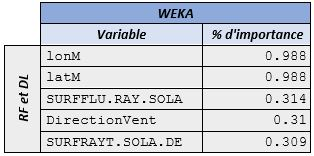
\includegraphics{img/ImpVweka.JPG}
    }
    \parbox{5cm}{
    \caption{ Variables importantes pour les algorithmes RF, et DL sous WEKA}
    \label{fig:wekaImp}
}
\end{figure}

 Le tableau illustré sur la figure \ref{fig:wekaImp} les variables importantes pour l’estimation de la visibilité horizontale avec les deux algorithmes \textit{Random Fores}t et \textit{Deep Learning} sous la plateforme \textit{WEKA}. Cette table montre que la pondération est la même pour les deux algorithmes.\\
 
 \ding{230} On constate que l'implémentation des algorithmes sous la plateforme \textit{WEKA} donne l'importance pour les mêmes variables lors du développement des algorithmes Datamining \textit{Random Forest} et \textit{Deep Learning}. Ainsi, la position géographique (latM et lonM) vient en tête des paramètres importants et ceci peut être justifié par le fait qu'on est en train d'étudier un problème de régression à caractère spatial. En fait, on cherche à estimer la visibilité sur un large domaine. Ensuite, on trouve deux paramètres importants et qui impactent largement l'occurrence de la visibilité réduite (vent et rayonnement).\\
 
Le tableau illustré sur la figure \ref{fig:impVar} dresse les cinq variables les plus importantes pour l’estimation de la visibilité horizontale avec les trois algorithmes ensembliste \textit{Random Forest}, \textit{Gradient Boosting Machine} et \textit{XGBoost} en utilisant les plateforme \textit{Scikit-learn} et \textit{H2O}. Il est à noter que pour le \textit{Deep Learning}, seule la plateforme \textit{H2O} offre la possibilité de mettre en évidence l'importance des variables en entrée.

\begin{figure}[!h]
    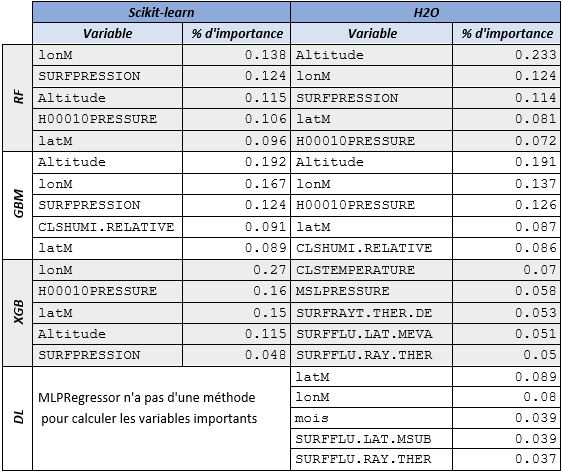
\includegraphics{img/ImpV.JPG}
    \caption{Variables importantes des algorithmes RF, GBM et XGB sous Scikit-learn et H2O}
    \label{fig:impVar}
\end{figure}

\ding{230} On constate que l'implémentation des algorithmes sous la plateforme \textit{H2O} et \textit{Scikit-learn} donne l'importance pour diverses variables lors du développement des algorithmes Datamining. Ainsi, on retrouve souvent la position géographique (latM, lonM, AltM et surface) et ceci peut être également justifié par le fait qu'on est en train d'étudier un problème de régression à caractère spatial. En fait, on cherche à estimer la visibilité sur un large domaine. Ensuite, on trouve des paramètres importants et qui impactent largement l'occurrence de la visibilité réduite à savoir les température et l'humidité à 2m ainsi que la pression au niveau de la surface et le rayonnement.\\



